\documentclass[11pt,spanish]{article} % Tipo y tamaño de letra del documento.


\usepackage[utf8]{inputenc}
\usepackage{subfiles}
\usepackage{biblatex}
\addbibresource{references.bib}
\usepackage{multicol}
\usepackage{amsfonts}
\usepackage{blindtext}
\usepackage{mathrsfs}
\usepackage{amsmath}
\usepackage{siunitx}
\usepackage{centernot}
\usepackage[shortlabels]{enumitem}
\usepackage{subfig}
\usepackage{datetime}
\usepackage{listingsutf8}
\usepackage[spanish]{babel}
\usepackage{tikz}
\usepackage{hyperref}
\usepackage[vlined,ruled,linesnumbered]{algorithm2e}
\usepackage{listings}
\usepackage{float}
\usepackage{url}
\usepackage{csquotes}
\usepackage{fourier} %font
\usepackage[top=2cm, bottom=2cm, left=2.5cm, right=2.5cm]{geometry}
\usepackage{pgfplots}
\usepackage{fancyhdr}
\usepackage{mdframed}
\usepackage{tikzducks}
\usepackage[nameinlink]{cleveref}
\usepackage{epigraph} 

\pgfplotsset{compat=1.18}

\usetikzlibrary{shapes.arrows, shapes.geometric, arrows.meta,angles,quotes,positioning,arrows,fit,quotes,calc}
\tikzset{>=latex} 

\setlength\algomargin{1em} 
\SetFuncSty{sc} 
\SetCommentSty{em} 


\Crefname{figure}{Fig.}{Figs.}
\newcommand\crefrangeconjunction{--}
\Crefname{table}{Tabla}{Tablas}
\Crefname{subsubsection}{Subsubsec.}{Subsubsections}
\Crefname{subsection}{Subsec.}{Subsections}
\Crefname{section}{Sec.}{Sections}
\Crefname{equation}{eq.}{eqs.}
\crefname{thm}{Theorem}{theorems}
\Crefname{thm}{Theorem}{Theorems} 

\definecolor{algoco}{rgb}{0,0.0,1}

\hypersetup{
  colorlinks=true,
  linkcolor=algoco,
  citecolor=blue,
  urlcolor=blue,
}

\lstset{
extendedchars=true
inputencoding=utf8/latin1,
basicstyle=\footnotesize\sffamily\color{black},
commentstyle=\slshape \color{gray},
numbers=left,
numbersep=10pt,
numberstyle=\tiny\color{red!80!black},
keywordstyle=\color{red!80!magenta},
showspaces=false,
showstringspaces=false,
stringstyle=\color{cyan!80!black},
tabsize=2,
literate={á}{{\'a}}1 {é}{{\'e}}1 {í}{{\'i}}1 {ó}{{\'o}}1 {ú}{{\'u}}1,
frame = single, 
numbers = none,
float, floatplacement = ht, captionpos = b,
xleftmargin = 2em, xrightmargin = 2em, 
}

\newcommand{\ub}[1]{\underbrace{#1}}
\newcommand\tcm{\textcolor{blue}}
\newcommand\tca{\textcolor{algoco}}

\setlength\epigraphwidth{.7\textwidth} 

\newcommand{\tnum}{1} % reemplace 1 por el número de la tarea
\newcommand{\sem}{2025-1} % reemplace 2024-2 por el semestre correspondiente
\newcommand{\campus}{San Joaquín \\ Santiago} % reemplace Casa Central por el campus correspondiente
\newcommand{\rolusm}{202173574-7} % reemplace 2025073100-1 por su rol
\newcommand{\namestudent}{Benjamín Daza Jiménez} % reemplace Al Goritmo Pérez por su nombre
\newcommand{\deadline}{21 de abril de 2025 } % reemplace 26 de abril de 2025, medio día por la fecha de entrega

\headheight=14pt
\linespread{1.3}
\author{\namestudent}
\pagestyle{fancy}
\fancyhf{}%
\fancyfoot[R]{ \namestudent \\ \rolusm}
\fancyfoot[L]{Campus \campus} 
\fancyfoot[C]{\thepage}
\rhead{\sem}
\lhead{INF-221}
\renewcommand{\headrulewidth}{0.4pt}
\renewcommand{\footrulewidth}{0.4pt}
\newbool{programs}
\boolfalse{programs}
\chead{REPORTE TAREA \tnum~}



\title{
  \huge
  \textbf{REPORTE TAREA \tnum~ \\ ALGORITMOS Y COMPLEJIDAD} \\[1ex]
  \emph{\textquote{Más allá de la notación asintótica: Análisis experimental de algoritmos de ordenamiento y multiplicación de matrices.}} 
  }

  
\date{
  \small
  \today\\
  \currenttime
}




\begin{document}
\maketitle
\thispagestyle{fancy} 
\vspace{-1.0\baselineskip}




\begin{abstract}
  \textit{ 
    Se realizará un análisis mediante la implementación de algoritmos de ordenamiento y algoritmos de multiplicación de matrices, utilizando distintos datasets para ejecutar pruebas y obtener resultados comparativos. ¿Realmente existe una diferencia entre estas implementaciones? Los resultados se presentarán mediante gráficos que permitan visualizar claramente las diferencia entre los algoritmos analizados. Finalmente, este análisis permitirá obtener una visión más objetiva de cómo influyen estos algoritmos en operaciones que puedan ser comunes en distintos contextos computacionales.

  }
     
\end{abstract}

\setcounter{tocdepth}{1}
\tableofcontents


\newpage
\section{Introducción}
La eficiencia de los algoritmos es un factor fundamental para el rendimiento de las aplicaciones. El objetivo de este informe es implementar cuatro tipos de ordenamiento y dos tipos de multiplicación de matrices, con el fin de contrastar su rendimiento en distintas pruebas exhaustivas con conjutos de datos de tamaño variable, teniendo una visión completa de cada algoritmo.\\
Los algoritmos considerados para el análisis de ordenamiento son:
\begin{itemize}
    \item Selection Sort: algoritmo que ordena una lista buscando el menor (o mayor) elemento de cada pasada, colocándolo en su posición correcta.
    \item Merge Sort: algoritmo que divide el arreglo en mitades iguales hasta que queden subarreglos de 1 elemento, los fusiona en orden, comparando pares de elementos.
    \item Quick Sort: algoritmo que elige un pivote, luego reordena el arreglo dejando a los elementos menores al pivote a la izquierda y los mayores a la derecha. Se aplica recursivamente a los subarreglos.
    \item Función Sort de c++: Combina Quick Sort, Heap Sort e Insertion Sort, adaptándose al tipo de dato.
\end{itemize}
En cuanto a la multiplicación de matrices se evaluará:
\begin{itemize}
    \item Algoritmo de Naive: multiplica matrices siguiendo la definición clásica de la multiplicación.
    \item Algoritmo de Strassen: divide cada matriz en 4 submatrices. Calcula 7 productos especiales y los usa para construir la matriz resultado.
\end{itemize}
Se espera que los tiempos de ejecución de la función Sort de c++, Merge Sort y Quick Sort sean similares en la mayoría de los casos, ya que estos algoritmos comparten una complejidad promedio de O(n log n). Sin embargo, se anticipa un tiempo mucho mayor para el algoritmo de Selection sort, debido a su complejidad cuadrática. Para la multiplicación de matrices, se espera el algoritmo de Strassen sea más rápido que el algoritmo de Naive, ya que posee una complejidad menor al cúbico. \\
Se busca comprobar que los algoritmos de ordenamiento y de multiplicación de matrices presentan diferencias significativas en sus tiempos de ejecución, especialmente al trabajar con datasets de gran tamaño. Esto permitirá evidenciar cómo la eficiencia algorítmica impacta directamente en el rendimiento computacional a mayor escala.


\newpage
\section{Implementaciones}
En el siguiente url se ecnuentra el repositorio con los algoritmos trabajados.
\begin{mdframed}
    \begin{center}
        {\Large \url{https://github.com/Benjamin-Daza-Jimenez/INF221-2025-1-TAREA-1-master}}
    \end{center}
\end{mdframed}




\newpage
\section{Experimentos}
Los casos de prueba realizados fueron ejecutados en un notebook con procesador Intel Core i5-13420H a 2.10GHz, 16GB de memoria RAM DDR4 y almacenamiento SSD NVMe. Las pruebas se realizaron en un entorno de Windows 11 versión 10.0.26100 de 64bits, ejecutado solamente desde el equipo mencionado, permitiendo obtener mediciones comparables en cuando al rendimiento de los algoritmos analizados.
\subsection{Dataset (casos de prueba)}
Los datasets para algoritmos de ordenamiento de un arreglo unidimensional están compuestos de números enteros almacenados en archivos de nombre \{n\}\_\{t\}\_\{d\}\_\{m\}.txt\:
\begin{itemize}
    \item n hace referencia a la cantidad de elementos, pertenecuenco al conjunto N = \{$10^1$,$10^3$,$10^5$,$10^7$\}.
    \item t hace referencia al tipo de matriz, perteneciendo al conjunto T = \{ascendente, descendente, aleatorio\}.
    \item d hace referencia al conjunto dominio de cada elemento del arreglo d = \{D1,D7\}, donde D1 implica que el dominio es \{0,1,2,...,9\} y D7 implica que el dominio es \{0,1,2,...,$10^7$\}.
    \item m hace referencia a la muestra aleatoria y pertenece al conjunto M=\{a,b,c\}
\end{itemize}

Los datasets para algoritmos de multiplicación de matrices cuadradas están compuestos de n números en n filas almacenados en archivos de nombre \{n\}\_\{t\}\_\{d\}\_\{m\}\_1.txt y \{n\}\_\{t\}\_\{d\}\_\{m\}\_2.txt\:
\begin{itemize}
    \item n hace referencia a la dimensión de la matriz (n filas y n columnas) y pertenece al conjunto N = \{$10^4$, $10^6$, $10^8$, $10^{10}$\}.
    \item t hace referencia al tipo de matriz, y pertenece al conjunto T = \{dispersa, diagonal, densa\}. 
    \item d hace referencia al conjunto dominio de cada coeficiente de la matriz d = \{D0,D10\}, donde D0 implica que el dominio es \{0,1\} y D10 que el dominio es \{0,1,2,3,...,9\}.
    \item m hace referencia a la muestra aleatoria y pertenece al conjunto M = \{a,b,c\}.
\end{itemize}

Tener una variedad de datasets es importante para evaluar correctamente algoritmos de ordenamiento y para la multiplicación de matrices. El tamaño y dimensiones del conjunto de datos permite analizar cómo escalan con el tiempo los algoritmos. A su vez, la distribución de los datos afecta al rendimiento, especialmente en algoritmos que dependen de comparaciones o tienen estructuras distintas. Además, algunos algoritmos funcionan bien con datos ordenados, pero mal con otros casos. La aleatoriedad nos asegura que el algoritmo no esté optimizado para un paso en particular, teniendo una evaluación más completa.

\subsection{Resultados}
Para visualizar los resultados ejecutados en otro equipo, se debe realizar “make run” desde:
\begin{itemize}
    \item \texttt{../code/matrix\_multiplication} -> ejecutar multiplicación de matrices.
    \item \texttt{../code/sorting} -> ejecutar ordenamiento.
\end{itemize}

Al terminar la ejecución, los resultados estarán en:
\begin{itemize}
    \item \texttt{../code/matrix\_multiplication/data/matrix\_output} -> contiene carpetas (naive y strassen) con los resultados de las multiplicaciones en archivos de texto.
    \item \texttt{../code/sorting/data/array\_output} -> contiene carpetas (mergesort, quicksort, selectionsort y sort) con los resultados de los ordenamientos en archivos de texto.
\end{itemize}

Además, se pueden revisar los tiempos y el uso de memoria en:
\begin{itemize}
    \item \texttt{../code/matrix\_multiplication/data/measurements} -> archivos de texto para cada implementación de multiplicación de matrices.
    \item \texttt{../code/sorting/data/measurements} -> archivos de texto para cada implementación de ordenamiento.
\end{itemize}

Cabe destacar que la ejecución de estos algoritmos puede arrojar resultados distintos en cada implementación, ya que se generan nuevos datasets tanto para la multiplicación de matrices como para el ordenamiento. Además, el hardware del equipo en que se ejecuten los programas influye significativamente en el desempeño en términos de tiempo y memoria. No obstante, la tendencia general de los resultados no debería verse alterada, permitiendo replicar el análisis presentado en este informe sin modificar las conclusiones teóricas.

\newpage
Para el análisis de los algoritmos de ordenamiento, se realizaron pruebas utilizando distintos datasets, lo que permitió ampliar el estudio sobre su comportamiento. Inicialmente, como se muestra en la \autoref{fig:Figura1}, los tiempos de ejecución fueron similares hasta datasets de tamaño 100.000, donde comienza a evidenciarse una diferencia considerable en el tiempo requerido por selectionsort, y una leve diferencia respecto a quicksort.\\
Al aumentar las pruebas a datasets con 10.000.000 de elementos, se observa claramente el desempeño de mergesort y sort. Es importante señalar que no se realizaron pruebas con quicksort en estos últimos datasets debido a errores de segmentation fault en cada archivo, ni con selectionsort, dado que su ejecución supera las 5 horas de ejecución por archivo.\\


\begin{figure}[H]
    \centering
    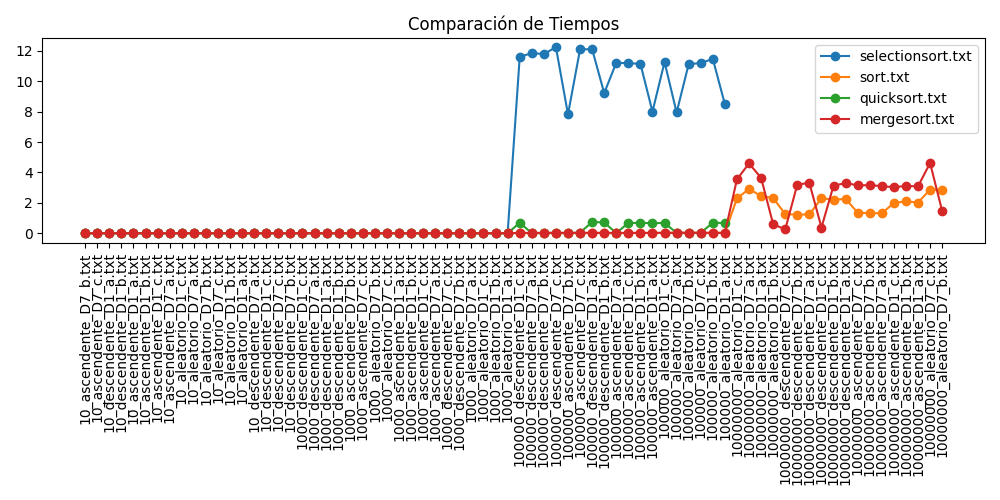
\includegraphics[width=\textwidth]{../code/sorting/data/plots/Grafico_tiempos.png}
    \caption{Tiempo en segundos empleado por cada ordenamiento}
    \label{fig:Figura1}
\end{figure}

\newpage
El uso de memoria para los archivos fue similar en todos los casos analizados hasta los datasets de tamaño 100.000 como se puede observar en la \autoref{fig:Figura2}. No obstante, no fue posible comparar el uso de memoria de quicksort y selectionsort en datasets de 10.000.000 elementos, ya que no se realizaron dichas pruebas. En particular, quicksort presentó errores de segmentation fault en todas las ejecuciones con estos últimos datasets, debido a que el uso de memoria superó el límite de stack asignado por el sistema. Esta situación se explica por la gran cantidad de llamadas recursivas provocadas por una mala elección de pivotes, generando una gran profundidad en la recursión.\\

\begin{figure}[H]
    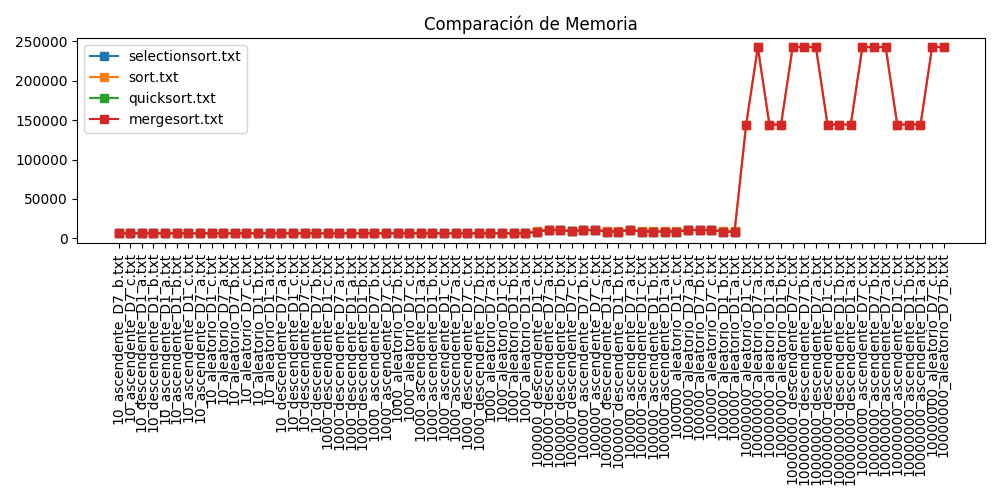
\includegraphics[width=\textwidth]{../code/sorting/data/plots/Grafico_memoria.png}
    \caption{Memoria en kilobytes utilizada por cada ordenamiento}
    \label{fig:Figura2}
\end{figure}

\newpage
Para el análisis de los algoritmos de multiplicación de matrices se realizaron pruebas utilizando distintos datasets, lo que permitió ampliar el estudio sobre su comportamiento. Como se observa en la \autoref{fig:Figura3}, los tiempos de ejecución fueron similares para ambas implementaciones en los primeros tamaños de matrices. Sin embargo, a partir de matrices de tamaño 1024×1024, el algoritmo de Strassen aumentó significativamente el tiempo de ejecución, lo cual resulta curioso considerando que, teóricamente, su orden de complejidad es menor que el de naive. Esto se explica porque Strassen realiza muchas operaciones costosas que no son eficientes para datasets relativamente pequeños. Se proyecta que los resultados favorables para Strassen se observarán en matrices de tamaño aún mayor, donde naive incremente considerablemente sus tiempos de ejecución.\\

\begin{figure}[H]
    \centering
    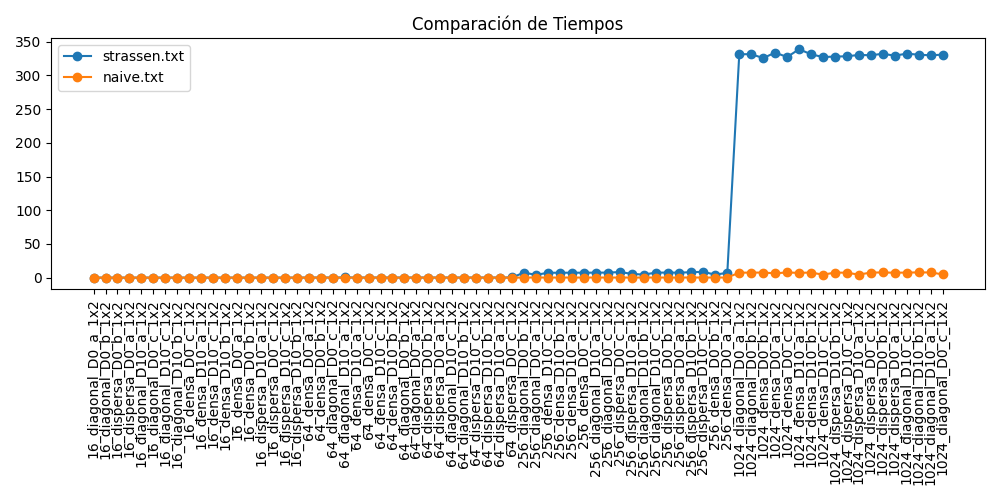
\includegraphics[width=\textwidth]{../code/matrix_multiplication/data/plots/Grafico_tiempos.png}
    \caption{Tiempo en segundos empleado por cada multiplicación}
    \label{fig:Figura3}
\end{figure}

\newpage
El uso de memoria para los archivos fue similar en todos los casos analizados, como se observa en la \autoref{fig:Figura4}. Se observa una leve diferencia en el consumo de memoria por parte de strassen, se debe a las operaciones internas adicionales que realiza en comparación con naive. No obstante, esta diferencia podría incrementar a medida que aumente el tamaño de los datasets.\\

\begin{figure}[H]
    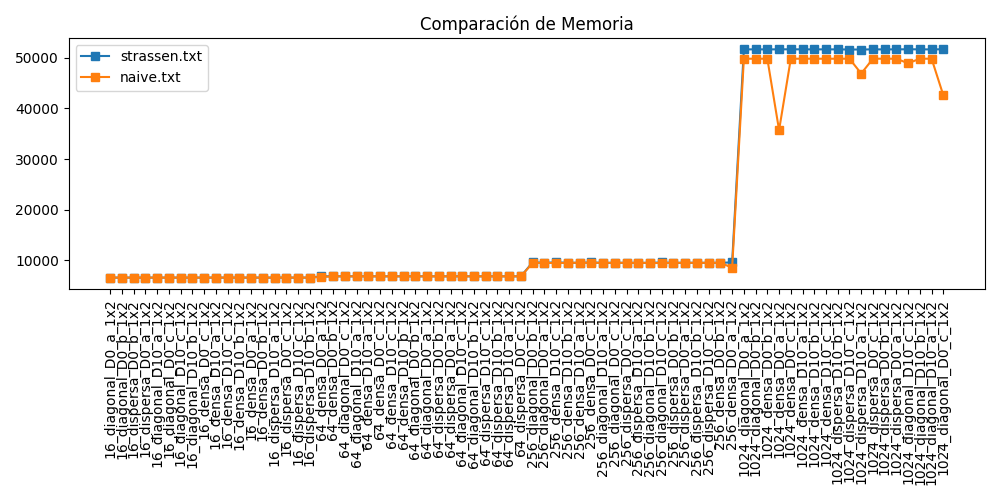
\includegraphics[width=\textwidth]{../code/matrix_multiplication/data/plots/Grafico_memoria.png}
    \caption{Memoria en kulobytes utilizada por cada multiplicación}
    \label{fig:Figura4}
\end{figure}

\newpage
\section{Conclusiones}
A partir de los datos generados y los tiempos obtenidos, se concluye que los algoritmos selectionsort y sort de C++ presentados en este informe son considerablemente más eficientes en tiempos de ejecución en comparación con SelectionSort y Quicksort en datasets de gran tamaño. Esta diferencia se debe a la forma en que están implementados, priorizando la división de tareas, la optimización de operaciones y una gestión más eficiente de grandes volúmenes de datos.\\
La complejidad temporal de estos algoritmos juega un papel fundamental en su desempeño. Mientras que los algoritmos cuadráticos según \autocite{cormen2009}, como SelectionSort, tienen una complejidad de O($n^2$), lo que provoca un aumento significativo en los tiempos de ejecución con grandes volúmenes de datos, algoritmos como Quicksort, Selectionsort y el sort de C++ tienen una complejidad de O(nlog(n)), lo que reduce drásticamente el tiempo de ejecución. Esta diferencia en la tasa de crecimiento explica por qué los algoritmos más eficientes presentan tiempos de ejecución considerablemente menores, como se evidenció en los casos de prueba. En los resultados obtenidos, los algoritmos eficientes lograron tiempos de ejecución reducidos, a excepción de Quicksort, el cual mostró un uso de memoria excesivo.\\
Un aspecto curioso de los resultados es la diferencia en los tiempos de Quicksort, que mostró un mayor uso de memoria y tiempos de ejecución. Esto se debe a la mala elección del pivote, lo que genera un comportamiento cercano al peor caso O($n^2$), aumentando significativamente tanto el tiempo como la memoria utilizada.\\
Por otro lado, en la multiplicación de matrices, los resultados son contrarios a lo esperado. A pesar de que el algoritmo de Strassen tiene un orden de O($n^{2.81}$), se esperaban tiempos de ejecución menores que los de naive el cual tiene un orden de $O(n^3$). Sin embargo, las diferencias en los tiempos se deben a que Strassen realiza más operaciones que el método tradicional, ya que incluye la división de matrices en submatrices y la combinación de resultados, lo que genera una sobrecarga y reduce su eficiencia. Por lo tanto, Strassen es más efectivo para matrices mucho más grandes que las que se probaron en este informe.\\
Finalmente, al realizar el análisis de los métodos de ordenamiento de datos y multiplicación de matrices, se concluye que cada método tiene sus propias ventajas y desventajas, y su eficiencia puede variar según las circunstancias y datos medidos. Comprender estas características nos permitirá escoger el algoritmo más adecuado según las necesidades específicas para la implementación.

\newpage

\newpage
\appendix


\section{Apéndice 1}
\input{sections/appendix1}
\printbibliography

\end{document}


